\documentclass[tikz,border=8pt]{standalone}
\usepackage{tikz}
\usepackage{amsmath, amssymb}

\begin{document}

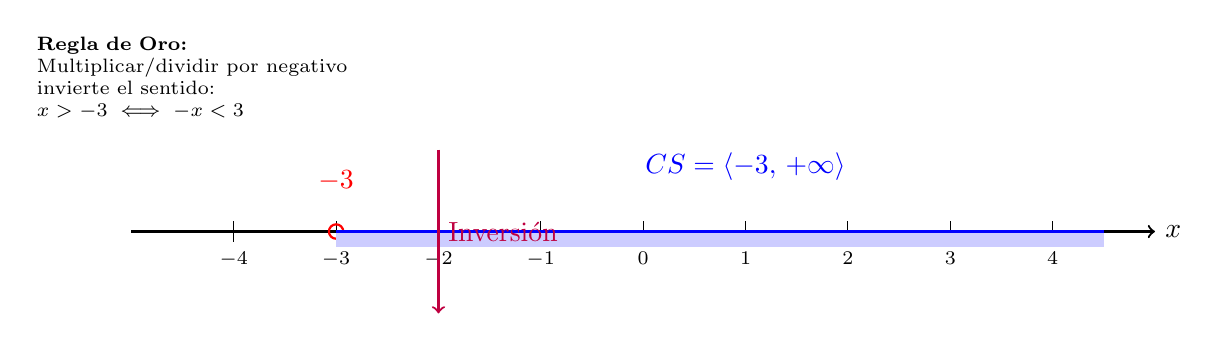
\begin{tikzpicture}[scale=1.3]

  % Recta numérica
  \draw[->, thick] (-5,0) -- (5,0) node[right] {$x$};
  \foreach \x in {-4,-3,-2,-1,0,1,2,3,4}
    \draw (\x,0.1) -- (\x,-0.1) node[below] {\scriptsize $\x$};

  % Punto crítico x = -3 (abierto)
  \draw[red, thick] (-3,0) circle (2pt);
  \node[red, above] at (-3,0.3) {$-3$};

  % Sombreado de CS = ⟨-3, +∞⟩
  \fill[blue!20] (-3,0) -- (4.5,0) -- (4.5,-0.15) -- (-3,-0.15) -- cycle;
  \draw[blue, thick] (-3,0) -- (4.5,0);

  % Etiqueta del conjunto solución
  \node[blue, above] at (1,0.4) {$CS = \langle -3,\,+\infty\rangle$};

  % Regla de signo: multiplicar por negativo invierte
  \node[align=left, text width=5cm, font=\scriptsize] at (-4, 1.5) {
    \textbf{Regla de Oro:}\\
    Multiplicar/dividir por negativo\\
    invierte el sentido:\\
    $x > -3 \iff -x < 3$
  };

  % Ejemplo visual: flecha invertida
  \draw[->, thick, purple] (-2,0.8) -- (-2,-0.8);
  \node[purple, right] at (-2,0) {Inversión};

\end{tikzpicture}

\end{document}
